\chapter{Single top quark production with a photon in the Standard Model}
\section{A brief overview of the standard model}
\section{The \texorpdfstring{$tq\gamma$}{tqGamma} process in the standard model}


\chapter{Measurement of \texorpdfstring{$tq\gamma$}{tqGamma}}
\textbf{TO DOS:}
\begin{enumerate}
    \item Define pseudorapidity in \ref{sec:atlas}
    \item \ref{sec:reconlepton} and \ref{sec:reconphoton} missing
    \item Cite anti-$k_t$ algorithm and study of misidentified jets in \ref{sec:jets}
    \item Define coordinate systems
\end{enumerate}


\section{The ATLAS Experiment}
\label{sec:atlas}
The European Organization for Nuclear Research, known as CERN, located in Geneva, has various experiments studying elementary particles through the collision of heavy ions and protons. 
The Large Hadron Collider (LHC), the particle accelerator of CERN, has a circumference of $27 \si{\kilo\metre}$ and can collide particles with an energy of up to $13.6 \si{\tera\electronvolt}$. 


The LHC consists of four extensive experiments: the ALICE, the LHCb, the CMS and the ATLAS experiments. The research in this paper is done with the help of the largest of these experiments, the ATLAS experiment. Figure 1 visualizes the structure of the ATLAS detector.  The detector is built symmetrically around the particle beam divided into three subdetectors.

The inner detector tracks charged particles just after the collision. It consists of three different systems of sensors in a magnetic field parallel to the beam. These sensors are the pixel detector, the semiconductor tracker that works with silicon strips and a transition radiation tracker to track particles with gas-filled tubes. 

In the EM calorimeter, metal layers (tungsten, copper or lead) absorb incoming particles and convert them into lower-energy particles called a shower. The calorimeters detect "showers" produced by electrons, photons and hadrons. 
Hadrons do not deposit all of their energy into the EM calorimeter; they get absorbed by steel layers in the hadronic calorimeter. 
Plastic scintillating tiles then produce photons that get converted into an electric current. 

The muon spectrometer measure trajectories of muons with the help of a magnetic field. The spectrometer detects muons in the range of $\bigl|\eta\bigr| = 2.7$. 
Monitored drift tubes measure for pseudorapidities up to $\eta = 2.0$ and cathode strip chambers fill higher pseudorapidities.  
\begin{figure}
    \centering
    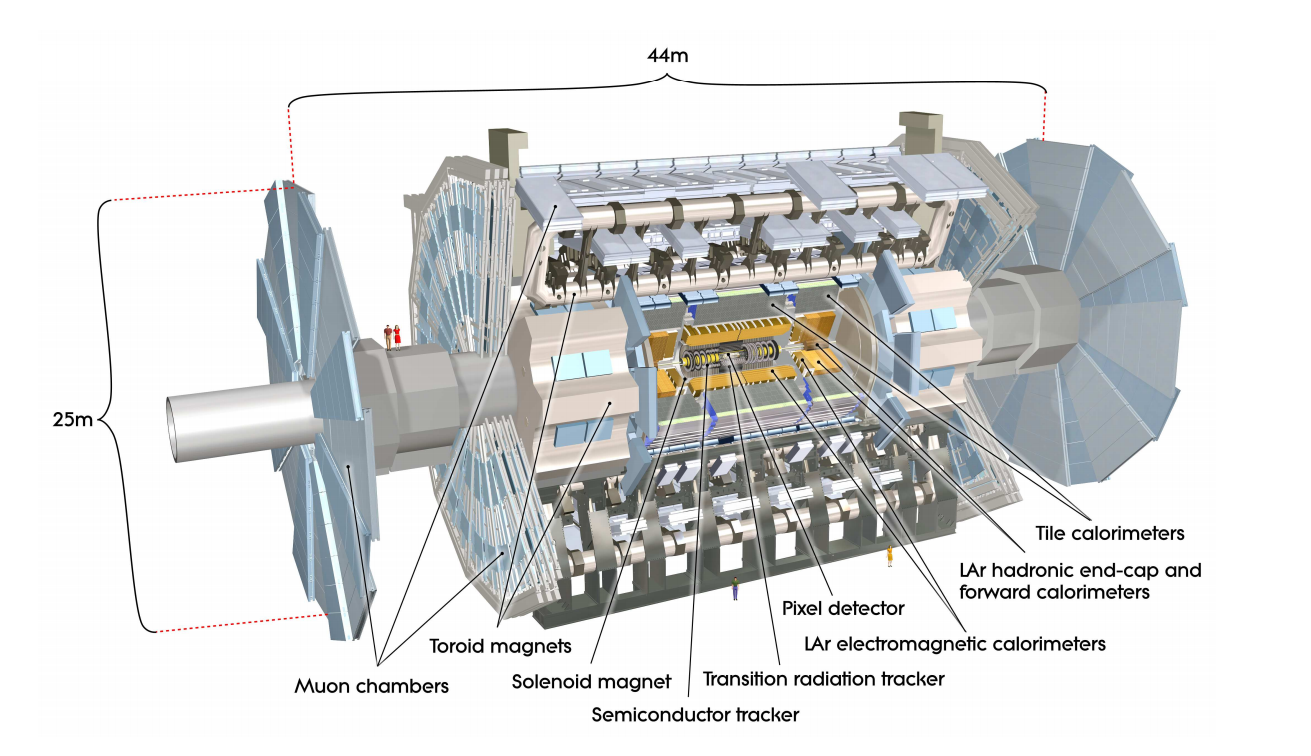
\includegraphics[width=0.9\textwidth]{Plots/atlasSCHEMA.PNG}
    \label{fig:atlasschema}
    \caption{Schematic visualisation of the ATLAS Detector \cite{Collaboration_2008}.}
\end{figure}



\section{Object Reconstruction at the ATLAS experiment}

\subsection{Reconstruction of photons}
\label{sec:reconphoton}
?
\subsection{Reconstruction of leptons}
\label{sec:reconlepton}
?
\subsection{Jets}
\label{sec:jets}
Jets are clusters of mostly mesons that result from the separation of two quarks. They are reconstructed with the help of the anti-$k_t$ algorithm \cite{anti_k_t} with a radius parameter of R = 0.4. 
This algorithm reconstructs jets by first identifying the particle source via the jet energy scale. It is then required that the jet has a transverse momentum of $p_T > 25 \si{\giga\electronvolt}$ and $\bigl|\eta\bigr| < 4.5$. 

Detector noise can lead to the misidentification of a jet. The nature of these misidentified jets has been studied thoroughly \cite{70} and a so-called "jet cleaning procedure" is used to tag them. 
Any event containing at least one "bad" jet is removed. 

\subsection{Missing transverse momentum \texorpdfstring{$E_T^{\text{miss}}$}{}}

If all particle products are considered, there should be no magnitude for the sum of the transverse momentum $p_T$ of all particles. 
Any measured magnitude is therefore attributed to an unmeasured particle. The missing transverse momentum $E_T^{\text{miss}}$ is consequently defined as the negative of this sum and assinged to a neutrino. 

\section{Background contributions from similar processes}



The criteria for event selection \ref{sec:eventselect} allow various different processes besides $tq\gamma$. These events contribute to the background noise. Any process that has similar decay products as tqGamma are background. 
The process $t\bar{t}\gamma$ holds the most similar decay product as it's products can be identical to the products of $tq\gamma$. Following processes is the production of a $W$-boson with jets, a $Z$-boson with jets and $t\bar{t}$. 
Table \ref{tab:background} lists these and the rest of the processes contributing to the background.
\begin{table}
    \centering
    \begin{tabular}{c c c}
        \toprule
        {} & Process \\
        \midrule
        1 & $tq\gamma$\\[.1cm]
        2 & $t\bar{t}\gamma$\\[.1cm]
        3 & $W\gamma + jets$\\[.1cm]
        4 & $Z\gamma + jets$\\[.1cm]
        5 & $t\bar{t}$\\[.1cm]
        6 & $s\-chan$\\[.1cm]
        7 & $t W$\\[.1cm]
        8 & $t\-chan$\\[.1cm]
        9 & $VV$\\[.1cm]
        10& $W+jets$\\[.1cm]
        11& $Z+jets$\\[.1cm]
        \bottomrule
    \end{tabular}
    \caption{List of SM processes that contribute to background noise in the measurement of $tq\gamma$.}
    \label{tab:background}
\end{table}



\chapter{Monte Carlo samples and event selection}
\section{Generation of Monte Carlo samples}
\section{Event selection}
\chapter{The Neural Network used for signal-background classification}
\section{Short introduction to neural networks}
\section{The neural network architecture}
\section{Input features for the neural network}
\section{Performance and distribution of the NN output}
\chapter{Differnetial analysis of the NN output}
%\chapter{Analysis of the effects of different event features on the neural network output}
\section{Correlations of input features with the NN output}
\section{NN output distribution dependence on photon \texorpdfstring{$p_T$}{pT} and fjet+photon energy}
\section{?}
\chapter{Conclusions}